\documentclass{ctuthesis}
\newcommand{\argmax}{\mathop{\mathrm{argmax}}}
\ctusetup{
	xdoctype = M,
	xfaculty = F3,
	mainlanguage = czech,
	title-english = {Scanner/Monitor of IoT radio networks},
	title-czech = {Přehledový přijímač / monitor rádiových sítí IoT},
	department-czech = {Katedra telekomunikační techniky},
	fieldofstudy-czech = {Komunikační systémy a sítě},
	author = {Ondřej Šulc},
	supervisor = {Ing. Pavel Troller, CSc.},
	supervisor-address = {Pestitelský ústav,\\ Zárivá 232,\\12000 Praha 2},
	month = 1,
	year = 2019,
	keywords-czech = {IoT, SDR-RTL, LoRa, Sigfox, Přehledový přijímač},
	keywords-english = {IoT, SDR-RTL, LoRa, Sigfox, Scanner},
	specification-file = {zadani.pdf}
}
\ctuprocess

\begin{abstract-english}
We develop \ldots
\end{abstract-english}

\begin{abstract-czech}
Rozvíjíme \ldots
\end{abstract-czech}

\begin{thanks}
Děkujeme \ldots
\end{thanks}

\begin{declaration}
Fakt sám \ldots
\end{declaration}
\usepackage{tabularx,array}
\usepackage{rotating}
\usepackage{booktabs}
\usepackage{multirow}
\begin{document}



\maketitle

\chapter{Úvod}

Foo bar
\chapter{Softwérově definované rádio}
\section{Úvod do SDR}
Značná část historie použití rádiových vln využívala rádia, která byla implementována čístě v hardware. Pro každou úpravu  vlastností rádia, tak bylo zapotřebí ho fyzicky upravit. S rozmachem výpočetní techniky však přišel vývoj i v oblasti rádia a na světlo světa se tak nejdříve dostala SCR (Software controled radio), která umožňovala v omezené míře ovlivňovat některé funkce a pozdějí i rádia SDR, která mohou být použita univerzálně díky digitálnímu zpracování signálu (DSP -Digital signal processing). \\
První známe nasazení SDR v praxi bylo v armádě, jednalo se o systém SPEAKeasy. Systém vyvinula DARPA v roce 1991 a umožňoval díky softwarové implementaci komunikovat prostřednictvím 10 různých vojenských protokolů na frekvencích od 2 MHz po 2 Ghz. SPEAKeasy byl připraven i na přidání dalších modulací a protokolů. O rok později již vyšel první článek o SDR na IEEE, napsal ho Joe Mitola a je tak považován za kmotra SDR. \ref{https://www.nutaq.com/blog/short-history-software-defined-radio-sdr-technology}\\
I přes tyto slibné začátky a podchycení jeho teoretických možností se SDR rozšiřovalo poměrně pomalu a jeho význam narostl až v podlední době s rozmachem levných výkoných integrovaných čipů. Velkou motivací využití SDR do budoucna jsou tzv. kognitivní rádia, která se dokáži přizpůsobit aktualnímu stavu spektra.
\section{Fungování SDR}
Základním znakem každého SDR je, že je značná jeho část realizována jako software běžící na programovatelném a configurovatelném HW zařízení. Toto zařízení můžeme nazvat rádiovou platformou (radio platform) a SW část jako aplikační rámec (aplication framework). Pokud je použitý jednotný standard tak tyto části mohou tvořit univerzální a znovupoužitelné komponenty a tak ušetřit prostředky a usnadnit jakékoliv upgrady.\\
Jedním z možných standardů je armádou používaná Softwarová komunikační architektura (Software Communication Architecture) vyvinutá  v programu JTRS (Joint Tactical Radio System). Tuto architekturu používá většina armádních SDR. \ref{Eged, B.; Babják, B. (2006) Universal Software Defined Radio Development Platform.}
Jinou možností je de facto standard pro rádio amatéry - GNU Rádio, kterému je v této práci věnována samostatná kapitola \ref{kapitola Gnu radio}.\\
Pokud na rádio nechceme koukat jako na krabičku ke které se připojí anténa, můžeme identifikovat jednotlivé funkční bloky:
\begin{enumerate}
\item
Převod z RF (rádiová frekvence) do IF (mezifrekvence)
\item
Převod do základního pásma
\item
Demodulace
\item
Uživatelské rozhraní
\end{enumerate}
Pokud se jedná o SDR můžeme ale zvolit i jednodušší vysokoúrovňový pohled a identifikovat tak tři prvky modelu: Zpracování analogového signálu (front-end), konverze domény (A/D, D/A) a digitální zpracování signálu (back-end), viz obrázek \ref{blokySDR}
\begin{figure}
\caption{Implementace rádia na základě SDR \ref{Eged, B.; Babják, B. (2006) Universal Software Defined Radio Development Platform}}
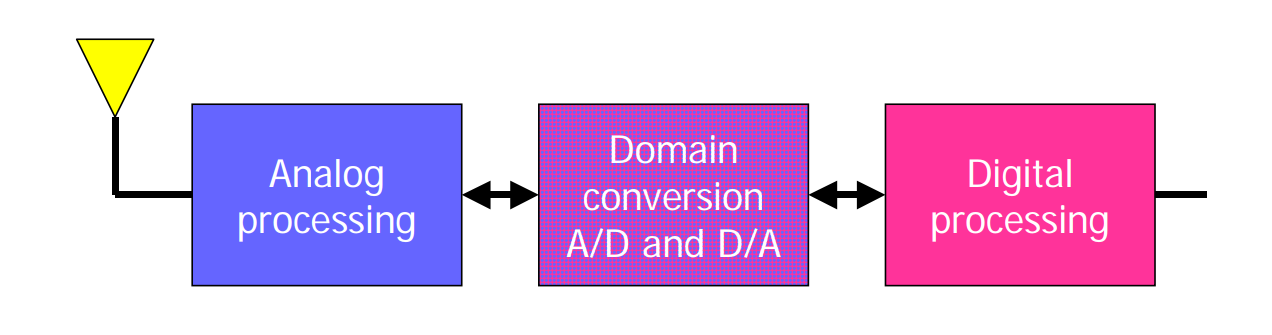
\includegraphics[width=1\textwidth]{./images/funkcniSDRbloky.png}
\label{blokySDR}
\end{figure}
\\
Fron-end se stará o převedení rádiového signálu na frekvenci a šířku pása, kterou dokáže zpracovat digítální back-end. Tvořé ho analogové zesilovače, směšovače filtry a oscilátory.\\
Konvertor domény jak již název napovída převádí anologový signál na digitální a obráceně. Souži mu k tomu vysokorychloostní širokopásmové A/D a D/A převodníky, jejich vlastnosti zásadně ovlivňují možnosti výsledného SDR. \\
 Poslední prvek tedy backend kde probíhá digitální zpracování je založen na FPGA a/nebo DSP programovatelných počítačích, na kterých běží software.\\
Převod mezi analogovou a digitální  doménou se může odehrát v různých místech zpracování viz obrázek  \ref{SDRconversion} a podle toho lze systémy kategorizovat.
\begin{figure}
\caption{Klasifikace SDR dle místa konverze domény\ref{bakalarka webrx}}
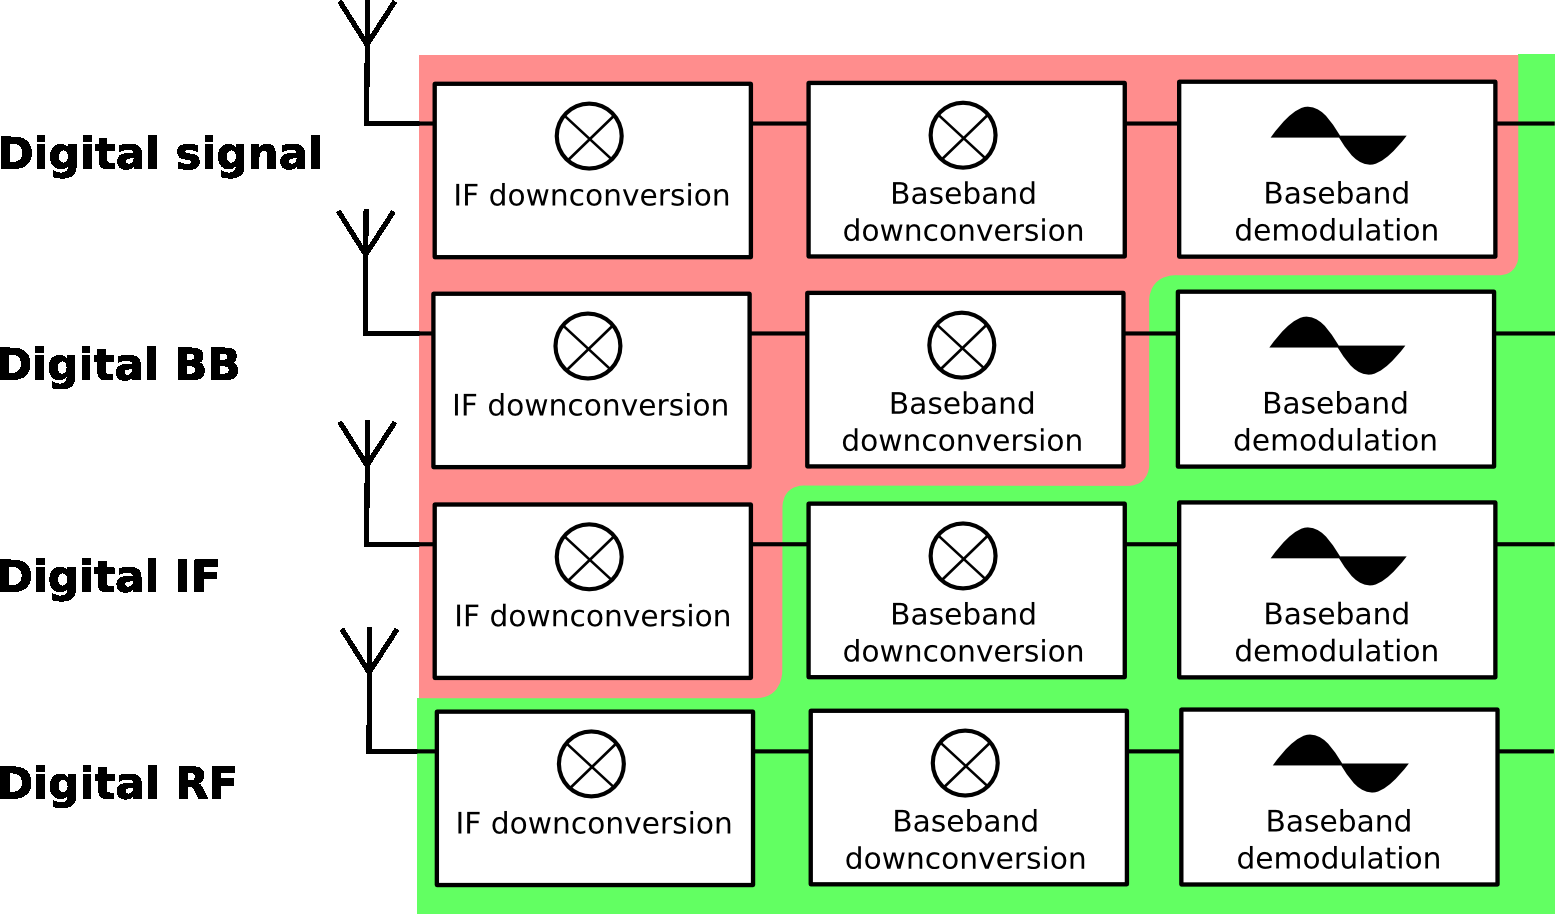
\includegraphics[width=1\textwidth]{./images/SDRconversion.png}
\label{SDRconversion}
\end{figure}
\begin{description}
\item[Digitální signál (Digital signal)]
V toto případě se v podstatě nejdná o SDR, vše je implementováno v HW. Výstupní signál je však digitální.
\item[Digitální základní pásmo (Digital Baseband)]
Zde se již část zpracování signálu odehrává v SW. Signál v základním pásmu je navzorkován a modulace se tak odehrává pomocí DSP. Podobné systémy požívají rádio amatéři například pro příjem BPSK31 pomocí rádiového přijímače a zvukové karty počítače na kterém běží SW pro demodlaci.
\item[Digitální mezifrekvence (Digital IF)]
V této kategorii probíhá vzorkování již na mezifrekvenci a předchází mu konverze z rádiové frekvence a filtrování implementované v HW. Podobné systémy jsou využívány radioamatéry nebo například v námořních rádiích, DSP zde slouží k filtrování šumu a demodulaci. 
\item[Digitální rádiová frekvence (Digital RF)]
I při vzorkování přímo RF je potřeba signál nejdříve zesílit a filtrovat až poté je možný jeho převod pomcí ADC. Následně probíhají všechny úkony již v SF. Příkladem systému z této kategorie může být HPSDR Mercury \ref{https://www.tapr.org/kits_merc.html} .
\end{description}
Toto rozdělení však nepočítá s přímou kvadraturní konverzí RF kde je vynechán mezikrok převodu na IF a převádí se rovnou na BB. V takovém případě se RF signál s reálnými hodnotami po zesílení a filtraci smíchá s výstupem oscilátoru s komplexním výstupem (sínus a kosínus), prožene fitrem dolní propust který odstraní vysoké frekvenční komponenty jako boční pásmo vzniklé smišením a poté navzrokuje dvěma ADC.\\
\begin{figure}
\caption{Blokové schéma SDR s přímou kvadraturní konverzí RF na BB\ref{http://www.ti.com/lit/ug/slwu085/slwu085.pdf}}
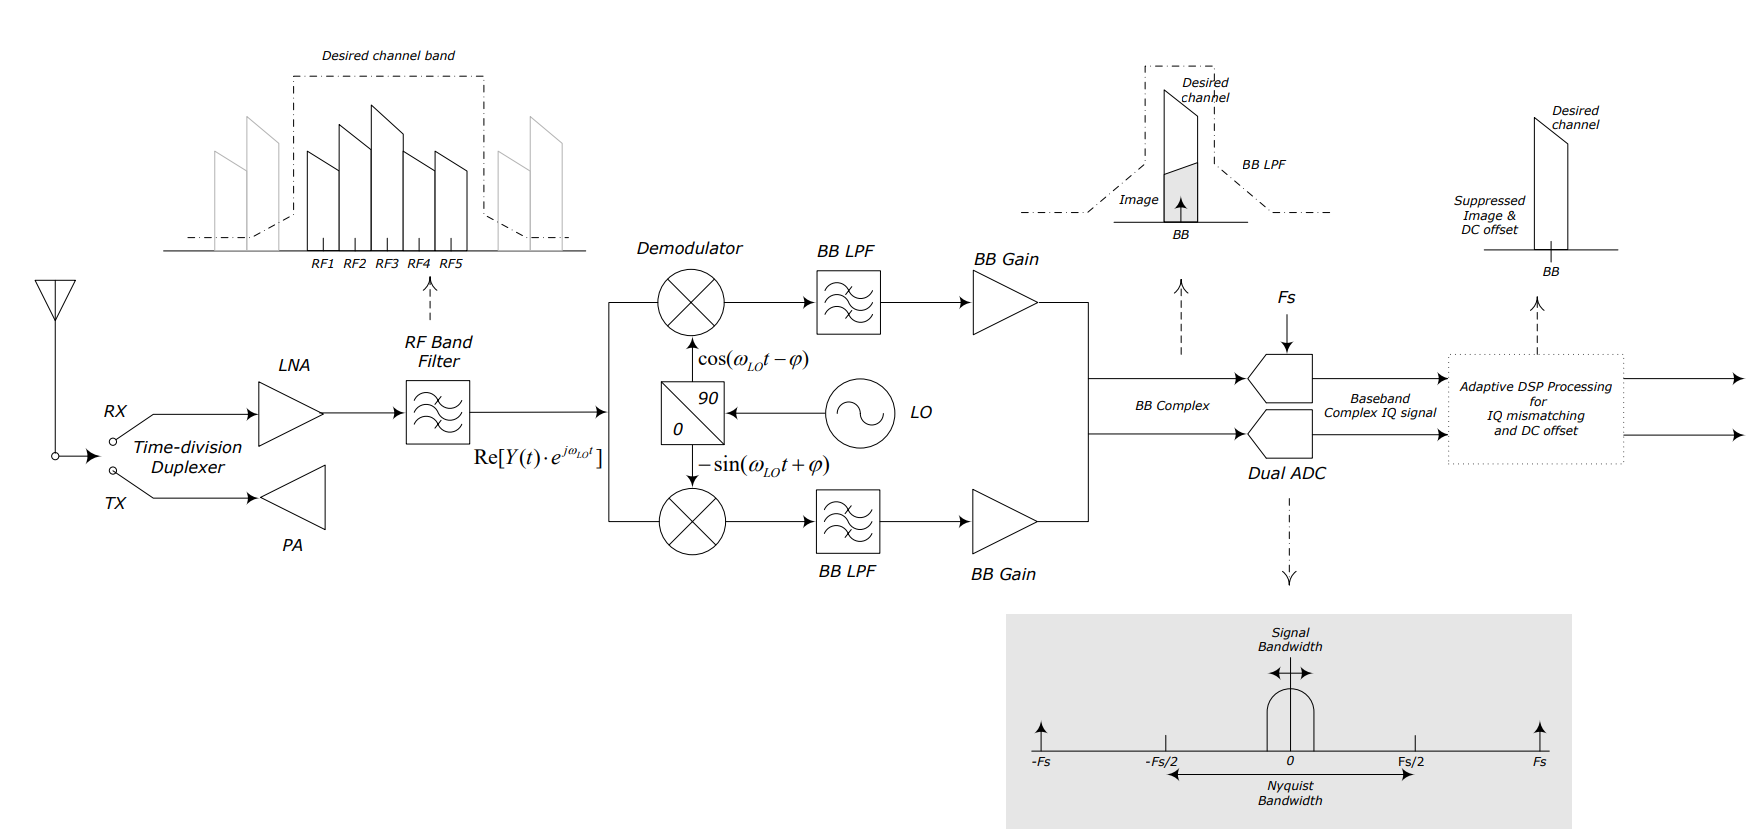
\includegraphics[width=1\textwidth]{./images/principSDR.png}
\label{principSDR}
\end{figure}
Popsaný postup je výhodný zejména díky své jednoduchosti, není potřeba filtrování IF a cena tak může být nižší. Další výhoda spočívá v tom, že Nyquistova vzorkovací fekvence pro komplexní I/Q signál je dvojnásobná oproti reálnému signálu a tak je možné vzorkovat mnohem širší pásmo.\\
Mezi nevýhody a také důvody proč se dříve používali slotižejší systémy patří možnost projevení se zrcadlového obrazu signálu a stejnosměrné složky v přijatém signálu. Zrcadlový obraz je způsoben rozdílem ve fázi a amplitudě mezi i a Q kanály. Tyto vady výrazně degradují přijatý signál avšak je možné je efektivně eliminovat korekcí rovnováhy IQ v digitálním zpracování.\\
Tento systém jsem takto podrobně rozepsal zejména protože ho používá většina dostupných SDR pro rádio amatéry včetně RTL-SDR použitého v této práci.
\\\\\\
Možnost přidat výhody a nevýhody http://www.winradio.com/home/facts.htm
\section{RTL-SDR}
Pokud si v minulosti chtěl někdo pořídit SDR musel počítat s částkami mnoha tisíc nebo i desítek tisíc korun a musel mít zároveň mít k dispozici velmi výkonný HW na kterém provádět výpočty. To se změnilo v roce 2012, kdy na scénu přišlo RTL-SDR - původně DVB-T USB tunner, který však s alternativními ovladači může být použit jako SDR a dá se pořídit za cenu do 500 kč.\\
Celé to začalo v roce 2008, kdy Realtek představil chipset RTL2832U s  DVB-T COFDM demodulátorem, hlavním učelem tohoto čipu a na něm postavených USB donglů byl příjem evropského standardu pro pozemní digitální televizní vysílání. Nabízel však i příjem digitálního rádia DAB a analogového FM. Tento malý detail se později stal velmi podstatným.\\
V roce 2010 totiž Eric Fry při pokusech o napsání ovladačů tohoto DVB-T donglu odposlouchával USB pakety během používání FM aplikace pro Windows. Eric zjistil, že narozdíl od přijmu DVB-T, kdy demodulace probíhá přímo na čipu, při příjmu FM, DAB a DAB+ demodulace probíhá až v SW počítače a přes USB se tedy přenáší I/Q vzorky, jeho primárním cílem však byli ovladače pro Linux a tak nezačal s vývojem pro použití jako SDR.\\
Informace se sice rozšířila, ale až do roku 2012 nenastal žádný větší pokrok. V tomto roce se o tento DVB-T přijímač od Realteku začal zajímat Antti Palosaari. Ten potvrdil možnost využití jako SDR díky přístupu k 8-bitovým I/Q vzorkům a začal s vývojem potřebného SW. Díky navázání spolupráce s organizací Osmocom, která se v té době vyvýjela vlastní SDR založené na tuneru E4000, což byl jeden z tunerů používaných v DVB-T přijímačích Realtek, práce nabrala obrátek a brzy byl vyvinut driver SW pro jednoduché použití těchto USB donglů jako SDR. Nejdůležitějším krokem bylo nejspíše vyvinutí ovladače pro linux, o to se v organizaci Osmocom postaral Steve Markgraf.
\ref{https://rtlsdr.org/#history_and_discovery_of_rtlsdr}
\ref{https://coherent-receiver.com/publications}
\\
Tento počin nastartoval éru RTL-SDR a na jeho základě tak vzniklo obrovské množství projektů všeho druhu, jmenovat budu jen pár těch zajímavějších (pokud čtete tu práci ve formátu PDF můžete kliknutím na projekt přejít na stránky, které se mu věnují):\\ \href{https://www.rtl-sdr.com/rtl-sdr-used-as-a-spectrum-analyzer/}{Spektrální analyzér}, \href{https://www.rtl-sdr.com/rtl-sdr-tutorial-analyzing-gsm-with-airprobe-and-wireshark/}{Odposlech GSM}, \href{https://www.rtl-sdr.com/adsb-aircraft-radar-with-rtl-sdr/}{Sledování letadel pomocí ADSB}, \href{https://www.rtl-sdr.com/using-rtl-sdr-cheap-entropy-source/}{Generátor nahodných čísel}, \href{https://www.rtl-sdr.com/receiving-weather-balloon-data-with-rtl-sdr/}{Příjem dat meterologických balónů}, \href{https://www.rtl-sdr.com/meteor-reflection-observations-with-rtl-sdr/}{Sledování meteoritů}, nebo \href{https://technet.idnes.cz/odposlech-site-tetra-a-mestske-policie-dhy-/tec_technika.aspx?c=A160913_145939_tec_technika_vse}{Odposlech vysílaček městské policie}\\

\section{Další dostupná SDR}
RTL-SDR je sice i v současné době to nejlevnější SDR, jeho kvalita však může být pro mnohá použití nedostatečná a tak v posledních letech vzniklo mnoho dalších dostupných SDR. Ta jsou sice o něco dražší, ale díky tomu, že jde o HW pro použití jako SDR navržený, mají větší rozsah, rozlišení, vzorkovací frekvenci a některá mohou kromě přijmu i vysílat.
\begin{description}
\item[USRP (Universal Software Radio Peripheral)]
USRP je celá řada produktů od společnosti Ettus Research. Hlavním vývojářem je Matt Ettus a první USRP spatřilo světlo světa již v roce 2008. V současnosti začínají ceny okolo 20 tisíc korun a v základu má USRP rozsah od 70 MHz po 6 GHz, tento rozsah však lze rozšířit pomocí přídavných desek. Starší hardware je uvolněn jako opensource a veškeré ovladače také. Z těchto důvodů jsou rádia USRP populární ve vědě, na universitách i mezi amatéry. USRP je kromě jiných podporované v GNU-Radio a Matlab SimuLinku a kromě příjmu zvládá i vysílat. \ref{https://www.ettus.com/about}
\item[bladeRF]
Již v roce 2012 v reakci na RTL-SDR začal vývoj bladeRF. Momentálně se nachazí již ve svojí druhé verzi a zajímavostí je, že jedna z variant obsahuje i FPGA pro HW akceleraci digitálního zpracování. Cena začíná na 11 tisích za verzi bez FPGA, verze s FPGA stojí 16 tisíc korum. 
\item[HackRF]
Toto SDR vyvinuté Michaelem Ossmanem v roce 2013 se díky úspěšné kampani na Kickstarter.com  začalo prodávat v roce 2014 a jeho cena je cca 7000 kč. Michael Ossman se již dříve proslavil vývojem zařízením pro odposlech bluetooth Ubertooth a HackRF navazuje jako další velmi kvalitní produkt. HackRF dokáže vysílat i přijímat a má rozsah má od 30 MHz po 6 GHz a zvládá i 2x2 MIMO. \ref{https://www.kickstarter.com/projects/mossmann/hackrf-an-open-source-sdr-platform}
\item[AirSpy]
AirSpy je asi nejlevněší alternativa k RTL-SDR a podobně jako ono neumí vysílat. Velkou popularitu AirSpy získalo zejména díky úzkému propojení s SDR\#  což je software pro analýzu a demodulaci rádiových signálů. V nejnovější verzi má rozsah od 24 MHz po 1,8 GHz a podporuje i externí hodiny pro použití vyžadující synchronizaci.
\ref{https://airspy.com/}
\end{description}


\begin{sidewaystable}[]
\begin{ctucolortab}
\begin{tabular}{c|cccccc}
\bfseries
Název                   & USRP B205mini         & \multicolumn{2}{l}{bladeRF 2.0 Micro}    & HackRF One  & AirSpy R2 & RTL-SDR \\ \Midrule
Cena (Kč)               & 20 000                & 11 000              & 16 000             & 7000        & 5000      & 500     \\
Frekvenční rozsah (MHz) & 70-6000               & \multicolumn{2}{l}{47-6000}              & 1-6000      & 24-1700   & 24-2200 \\
ADC rozlišení (bits)    & 12                    & \multicolumn{2}{l}{12}                   & 8           & 12        & 8       \\
Šířka pásma (MHz)       & 56                    & 56                  &                    & 20          & 10        & 16      \\
Možnost vysílání        & Full Duplex           & \multicolumn{2}{l}{Full Duplex 2x2 MIMO} & Half Duplex & Ne        & Ne      \\
Přesnost hodin (PPM)    & 2                     & \multicolumn{2}{l}{0,26}                 & 30          & 0,5       & 85      \\
FPGA (kLE)              & Ne (dražší verze Ano) & 49                  & 301                & Ne jen CPLD & Ne        & Ne      \\ 
\end{tabular}
\end{ctucolortab}
\caption{Přehled dospuných SDR}
\label{tab:sdr}
\cite{https://kb.ettus.com/B200/B210/B200mini/B205mini, https://www.rtl-sdr.com/review-airspy-vs-sdrplay-rsp-vs-hackrf/, https://www.itead.cc/airspy.html, http://www.taylorkillian.com/2013/08/sdr-showdown-hackrf-vs-bladerf-vs-usrp.html}
\end{sidewaystable}

\begin{table}
\begin{ctucolortab}
\begin{tabular}{cc}
\bfseries Foo & \bfseries Bar \\\Midrule
foo1 & bar1 \\
foo2 & bar2
\end{tabular}
\end{ctucolortab}
\caption{Foobar.}
\label{tab:foobar}
\end{table}

\chapter{LoRa}
\section{Fyzická vrstva (LoRa PHY)}
\subsection{Modulace}
Modulační schéma LoRa je založeno na Chirp Spread Spread Spectrum (Cvrlikající rozprostřené spektrum) modulaci  (Goursaud and Gorce, 2015) a definuje jeden “cvrk” jako jeden symbol  (Semtech, 2015a). Standardní nemodulovaný lineární cvrk se nazývá “základní cvrk” a může být matematicky popsán jako funkce času t takto (Mann and Haykin, 1991):
\begin{align}x(t)=e^{i(\varphi_{0}+2\pi(\frac{k}{2}t^{2} + f_{0}t))}
\label{eq:lora1}
\end{align}
Kde  $\varphi_{0}$ je počáteční fáze, $k$ je rychlost změny frekvence a $f_{0}$ je počáteční frekvence. Pokud je šířka pásma kanálu $BW$, tak parametry $f_{0}$ a $k$ jsou nastaveny tak, že se frekvence zvětšuje od $f_{0}-\frac{BW}{2}$ po $f_{0}+\frac{BW}{2}$ během periody $T$ cvrku. Tím pádem je $f_{0}=\frac{BW}{2}$ and $k = \frac{BW}{T}$. Doba trvání jednoho cvrku závisí na šířce pásma signálu a na parametru nazývaném činitel rozprostření (Spreading Factor - SF) dle vztahu $T = \frac{2^{SF}}{BW}$ (Seller and Sornin, 2014).
Vzhledem k tomu, že $x(t + nT) = x(t)$ kde $n\in \mathbb{N}$, celočíselná hodnota $i \in \{0, 1\}^{SF}$ může být namodulována na základní cvrk pomocí časového posunu $\hat{t} = Gray^{-1}(i)\frac{T}{2^{SF}}$ aplikovaného na signál ve vztahu \eqref{eq:mod1},  kde $Gray^{1}$ je dekódování Grayova kódu (Gray, 1953). Touto cestou je symbol v podstatě kvantovaný na $2^{SF}$ časových intervalů rozdělujích šířku pásma, nazýváme je “chipy” a právě ony určují $i$. Při příjmu modulovaného cvrku s neznámým časovým posuvem $x(t + \hat{t})$, může být hodnota cvrku zrekonstruována navzorkováním signálu vzorkovací frekvencí chipů a výpočtem:
\begin{align}i= Gray(arg \max (\lvert FFT(x(t+ \hat{t}) \odot \overline{x(t)}) \rvert ))
\label{eq:lora2}
\end{align}
Kde $\overline{x(t)}$ značí komplexně sdružený základní cvrk, $\odot$ značí multiplikaci po prvcích, $\lvert FFT(x) \rvert$ zančí velikost Rychlé Fourierovi transformace $x$, a $Gray$ je Grayovo kódování. 

\subsection{Prokládání}
Jako v každé jiné modulaci, musíme i zde počítat s chybami způsobenými šumem, interferencí, a časovými nebo frekvenčními posuny. Tyto chyby mohou způsobit, že hodnota čipu nebude dobře odečtena z modulovaného symbolu. Například poryv šumu může posunout vrchol v FFT spektru na jinou hodnotu chipu a tak jej znehodnotit.\\
Aby bylo možné minimalizovat dopad poryvů šumu na chybu jen jednoho bitu v symbolu je použito prokládání. Několik chipů je dohromady vepsáno do mřížky $\{0,1\}^{SF x (4 + CR)}$, kde CR (Coding Rate) značí počet paritních bitů a nabývá hodnot 1 až 4. Pokud tedy bude použit $SF = 7$ a $CR =4$ dostaneme matici  $\{0,1\}^{7 x 8}$, příklad je na obrázku \ref{fig:lora1}. K sískání kódové slova je pak potřeba číst bity po diagonále matice. Na rozdíl od patentu LoRy (Seller and Sornin, 2014), kde se uvádí, že směr diagonálního čtení bitů z mřížky je směrem dolů, v praxi lze pozorovat opačný směr. Tímto způsobem tak první chip obsahuje všechny nejméně významné bity (LSB - Least significant) všech kódových slov, druhý čip všechny druhé bity všech slov a tak dále. Díky tomu v případě ztráty celého čipu dojde k chybě jen v jednom bitu na kódové slovo.\\
Dalším způsobem jak zvýšit odolnost proti rušení vysílání je použití módu redukované rychlosti (reduced rate mode). V případě použití tohoto módu jsou první dvě řady prokládací matice zahozeny a její rozměr se tak změní na $\{0,1\}^{SF-2 x (4 + CR)}$ což způsobí, že z ní nasledně vyčteme o dvě kódová slova méně. Zahozené řádky obsahují nejméně významné bity chipů, které jsou nachylnější k chybám protože odpovídají užším frekvenčním intervalům v FFT spektru. Z toho vyplývá, že mód redukované rychlosti obětuje rychlost přenosu dat ve prospěch odolnosti proti šumu. Hlavička fyzické vrstvy LoRa je v tomto módu vysílána vždy, kdežtkoo užitečná data je v případě použítí SF 11 nebo 12.

\subsection{Kódování}
Po přečtení kódových slov z prokládací matice mají tato délku $4 + CR$. Kvůli zamezení vzniku stejnosměrné složky byla slova v části rámce s užitečnými daty XOR-ována 9-bitovým lineární posuvným registrem se zpětnou vazbou (LSFR Linear feedback shift register) (whitening). A proto musí po synchronizaci projít stejným procesem znovu. Přesný algoritmus není v patentu určen a jeho výběr je tedy na každém výrobci zvlášť. \\
Na několika testovacích zařízeních \ref{nejdulzittejsipapir} reverzním inženýrstvým zjistilo použité upraveného $4/(4 + CR)$ Hammingova kódu. Ve výsledku tak z každého kódového slova po dekódování získáme 4 bity dat. Ta jsou pak naparsována du struktury rámce lora.

\subsection{Struktura rámce}
Na fyzické vrstě LoRa definuje rámec jako strukturu složenou z následujících polí. Pole jsou uvedena ve stejném pořadí jako v rámci.  (Semtech, 2015b, p. 27–29)
\begin{description}
\item[Preambule]
Sekvence základních cvrků, která slouží k časové a frekvenční synchronizaci. Počet cvrků není pevně dán.
\item[Symboly synchronizace rámce]
Dva modulované cvrky co mouhou být použity pro identifikaci sítě. Hardwarový přijímač zahodí rámcec, které obsahují synchronizační symboly co neodpovídají jeho nastavení.
\item[Symboly synchronizace frekvence]
Dva sdružené cvrky následované sdruženým cvrkem s periodoou $\frac{T}{4}$ určené pro přesnou frekvenční synchronizaci.
\item[Hlavička (nepoviná)]
Hlavička obsahuje délku užitečných dat, použitou přenosovou rychlost, indikuje použití Cyklického redundantního součtu (CRC - Cyclic redunduncy check) a jendobajtovou kontrolní sumu hlavičky. Pro modulaci hlavičky je vždy použito $CR =4$ a mód redukované rychlosti. Pokud hlavička vysílána není (implicitní mód) musí mít jak přijímač tak vysílač předem schodně nastavený CR a také zdali je použito CRC.
\item[Užitečná data]
Pole o proměnné délce obsahující data vrstvy přístupu k médiu (MAC - Media access control) a případné dvoubajtové CRC těchto dat.
\end{description}
\subsection{Struktura hlavičky}
Délka hlavičky není ve specifikaci nikdy přímo určena. Lze jí však vydedukovat z toho, že hlavička je vždy vysílána v módu redukované rychlosti, má $CR =4$ a SF minimálně 7. Z toho vyplívá že hlavička se musí vejít do mřížky $\{0,1\}^{7-2 x 8)}$ a to odpovídá 5 kódovým slovům. Každé slovo má 8 bitů a dohromady je to bitů 40. Jakékoliv zbývající bity jsou použity pro užitečná data. \\
Po dekódování díky redundantním bitům dostáváme $40\frac{4}{8} = 20$ bitů nebo 2,5 bajtu. V \ref{nejdulezitejsipapir} experimentálně vyzkoušeli pořadí hlavičky. První bajt udává délku datového obsahu, následuje půlslabika  udávající CR a přítomnost MAC CRC a poslední bajt obsahuje kontrolní součet hlavičky, z něj je však používá jen 5 LSB bitů.

\section{Softwarová demodulace}
\ref{nejdulezitejsipapir} dokázali implementovat kompletní PHY vrstvu LoRa ve frameworku GNU Radio. Jejich zdrojové kódy jsou open source a dostupné na Githubu. Funkčnost příjmu signálu LoRa mého scanneru vychází z jejich práce. V této kapitole je pospsán princip fungování.
\subsection{Detekce a synchronizace}
\label{subsec:detection}
Aby mohl být signál demodulován musí být nejdříve detekován. K tomu slouží preamule která má dva opakující se cvrky čehož dokáže využít použitý Schmidl-Cox algoritmus. Ten definuje dvě veličiny $P(d)$ a $R(d)$, ty jsou definované takto (Schmidl a Cox, 1997) \ref{SchmidlCox}:
\begin{align}P(d) = \sum_{m=0}^{L-1} (x_{t+m}^{\ast}x_{t+m+L})
\label{eq:lora3}
\end{align}
\begin{align}
R(d) = \sum_{m=0}^{L-1} \lvert{x_{t+m+L}}\rvert^{2}
\label{eq:lora4}
\end{align}
kde $L$ je délka symbolu, $t$ je index vzorku komplexnímo signálu $x$ a $x^{\ast}$ je jeho komplexně sdružený signál. Veličiny $P(d)$ a $R(d)$ jsou použity k výpočtu časové metriky $M(d)$:
\begin{align}
M(d) = \frac{\vert P(d) \rvert ^{2}}{R(d)^{2}}
\label{eq:lora5}
\end{align}
Časová metrika $M(d)$ v podstatě počítá normalizovanou autokorelaci délky $L$ přes dva symboly, maximum bude mít ve cvhíli kdy v signálu budou za sebou dva totožné symboly. Díky tomu, že oba symboly jsou chybami způsobenými prřenosem (interference, frekvenční odchylka nosné (CFO - Carrier frequency ofset), odchylka vzorkovací frekvence) ovlivněny stejně, tak tyto chyby téměř neovlivní výsledek korelace. Aby bylo možné efektivně počítat rovnice \ref{lora4} a \ref{lora5} v programu byla použita knihovna VOLK (Vector Optimized Library of Kernels), která implementuje SIMD (Single Instruction, Multiple Data) instrukce. Na obrázku \ref{fig6a} je vidět příklad výsledku použití časové metriky $M(d)$ na komplexním signálu LoRa. Kolem vzorku 2500 funkce dosahuje horní plošilny a poukazuje tak na existenci preambule. \\
I přesto že tento algorimus detekuje preambuli velmi dobře, není možné přesně určit počátek symbolu jen z horní plošiny časové metriky. Tým kolem Wanga \ref{wang et al} proto navrhl vylepšení kdy je od časové metriky $M(d)$ odečtena její opožděná verze $M_{2}(d)$, tím se z plošiny stává vrchol \ref{fig6b} a lze tak za začátek symbolu považovat vzorky odpovídající maximu této metriky. Nicméně ani to není jak je patrné z \ref{fig6c} dostatečně přesné pro signály LoRa.\\
Aby \ref{nejdulezitejsipapir} tenhle problém vyřešili museli vymyslet nové řešení. To se zakládá použití Schmidl-Coxovi metriky pro přibližné určení okna ve kterém se nachází druhý symbol preambule a následném zpřesnění pomocí ideálního lokálně vygenerovaného cvrku. Jeho okamžitá frekvence $\omega_{l}(t)$ a normovaná okamžitá frekvence signálu Lora  $\omega(t)$ jsou vzájemně korelovány (přes posuvné okno?) a index vzorku jež odpovídá maximální hodnotě této funkce je považován za počátek symbolu. Použití omažité frekvence místo komplexních hodnot je odůvodněno chybami CFO, které by bez korekce mohly ovlivnit přesnost synchronizace. Použitím okamžité frekvence jsou podobně jako u Schmidl-Coxova algoritmu tyto chyby zanedbatelné.
\begin{align}
symbol start = \argmax_{i \in \{0,1,...L\}} (\omega_{l} \star \omega)(i)
\label{eq:lora6}
\end{align}
Výsledek je na \ref{fig6d}. Poslední součástí tohoto řešení je určení prahové hodnoty maxima korelačního koeficientu okamžitých frekvencí lokálnlně gerovaného cvrku a přijátého. Pokud je tato hodnota menší než prahová je daný rámec zahozen, protože se buďto jedná o falešně pozitivní detekci rámce nebo o nepovedenou synchronizaci.
\subsection{Demodulace}
\label{subsec:demodulace}
Po úspěšné synchronizaci následuje fáze demodulace popsaná v předchozí kapitole. Oproti teorii má však v praxi FFT demodulace nevýhodu v tom, že je citlivá na odchylku frekvence, která způsobuje posun hodnot FFT a tím i odečítaných hodnot chipů. Tím pádem je potřeba přesná synchronizace frekvence, kterou je navíc potřeba aplikovat na každý kanál LoRa zvlášť. Separace kanálů a následná synchronizace každého z nich je však v softawaru příliš náročná operace a tak \ref{nejdulezitejsipapir} přišli s novou metodou demodulace, která je nezávislá na frekvenci a umožňuje demodulaci na všech kanálech současně v reálném čase. V porovnání s FFT metodou je však méně robustní.\\
Nejdříve je potřeba spočítat okamžitou úhlovou fekvenci $\omega[t]=\frac{d\varphi[t]}{dt}$. Poté je potřeba $\omega[t]$ vyhladit a decimovat konstantním decimačním faktorem $\frac{s_fT}{2^{SF}}$ kde $s_f$ je vzorkovací frekvence. Díky tomu je pak počet vzorků v $\omega[t]$ schodný s $2^{SF}$ následně je vypočítán digitální gradient $f$:
\begin{align}
D_t[\omega[t]] = \omega[t+1]-\omega[t]
\label{eq:lora7}
\end{align}
Tuto operaci si lze představit jako filtr horní propusť okamžité frekvence nebo jako druhou derivaci fáze. Protože frekvence základního cvrku se lineárně zvyšuje s $k$ - $\omega(t) = kt + f_0$ je její derivace $\omega'(t)$ rovna $k$. Pro modulované cvrky se však v $D_t$ objeví ostré šličky v místech přechodu mezi vysokou a nízkou frekvencí. Přítomnost takových špiček indikuje časový posun $\hat{t}$, nepřítomnost naopak idikuje časový posun 0 - základní cvrk.\\

Dalším problémem při demodulaci je zpožďování/předbíhání hodin v jednotlivých zařízeních. Kristalové oscilátory v LoRa vysílači a SDR se budou zákonitě navzájem předbíhat nebo zpožďovat, rozdíl jejich frekvencí je předem neznámý, ale v průbhu času se musí projevit. To může způsobovat problémy zejména v případě delšího datového obsahu v kombinaci s vyšším SF. V patentu LoRa jsou pro účely korekce tohoto jevu použity pilotní symboly, které pomohou sledovat časování. Ve skutečnosti se však zdá, že k jejich použití nebylo přistoupeno. Je tedy nutné využít techniku slepého odhadu, která využívá převzorkování přijatého signálu $N$-krát. Aby tato technika byla funkční je potřeba aby hodnota $N$ odpovídala následujícímu vztahu $\lvert\Delta t \rvert < \frac{N}{2}$\\, kde $\Delta t$ je chyba časování na symbol.
Prvním krokem je synchronizace popsaná v \ref{ subsec:detection}. Pokud je chyba časování na symbol  $\lvert\Delta t \rvert < \frac{N}{2}$\\, lze $\lvert\Delta t \rvert$ určit následujícím způsobem:
\begin{enumerate}
\item
Symbol je demodulován běžným způsobem jak je popsáno v \ref{subsec:demodulace} a je tak získána hodnoto chipu $i$  a časového posunu $\hat{t}$.
\item
Na přijímači je lokálně generovaný základni cvrk modulován na i což způsobí časový posun $\hat{t}_1$ lokálního signálu.
\item
Protože lokálně generovaný cvrk není ovlivněn rozdílem oscilátorů vysílače a přijímače můžeme vzájemné zpoždění oscilátorů definvat takto $\Delta t = \hat{t}_1 - \hat{t}$. Nyní stačí na příjimači opravit $\hat{t}$ připočtením vzájemného zpoždění k přijatému signálu.
\end{enumerate}
Již zmíněná podmínka $\lvert\Delta t \rvert < \frac{N}{2}$ je daná tím, že při jejím nesplnění dekodér špatně určí hodnotu chipu $i$ a chyba se tak bude šířit i do dalších symbolů. Hodnota $N$ tak není určena přímo ale jako interpolace z $\hat{t}$ do $\hat{t} + \Delta t$. Vyšší hodnoty $N$ by dále vylepšovali přesnost korekcí zpoždění ale také by zvyšovali náročnost výpočtu.

\subsection{Dekódování}
Ve fázi dekódování jsou hodnoty chipů zpětně proloženy a tím jsou získána kódová slova s 4 + CR bity. Prvních 8 kódových slov lze přímo dekódovat jako hlavičku fyzické vrstvy. Datový obsah však musí být nejprve XORován bělící posloupností. I přesto že dle výrobce LoRa Semtech má jít o sekvenci generovanou 9-bitovým LFSR ve skutečnosti je dle výzkumu \ref{Knight 2016, Blum 2017} použita posloupnost mírně odlišná, která však není veřejně zdokumentovaná.\\
Pokud však známe původní  kódové slovo i přijaté vybělené lze snadno zjistit sekvenci použitou pro XORování následovně
$w^{(j)} = c_w^{(j)} \oplus c^{(j)}$. Pro zjednodušení lze vyslat všechna kódová slova nulová a tím dostaneme rovnici $w^{(j)} = c_w^{(j)} \oplus 0$ a na výstupu tak máme přío samotnou bělící sekvenci, kterou můžeme uložit a poté náčítat z tabulky. \\
Po Odbělování příchází poslední krok a to Hammingovo dekódování kódových slov. U LoRa jsou datové bity umístěny na jiných pozicích než je běžné a to na indexech 0,1,2 a 3 bajtu místo indexů 1,2,3 a 5. Graficky je toto mapování zobrazeno na \ref{hamming}. Po extrakci datových bitů jsou pak pomocí paritních bitů detekovány a případně opraveny chyby a tím získána původní data.


\chapter{SigFox}
\section{Rádiový protokol Sigfox)}

Základním poznávacím znamením technologie Sigfox je pužití velmi úzkého pásma (UNB - Ultra Narrow Band). To dovoluje vysílání na větší vzdálenosti díky úzkému zaměření vysílacího výkonu každého zařízení. Navíc díky použití UNB může na jednom místě operovat velké množství zařízení bez přílišného vzájemného rušení. \\
Sigfox používá různá modulační schémata pro uplink a downlink, důvodem je optimalizace využití spektra. Různá je i šířka pásma, přenosová rychlost, vysílací výkon i struktura rámce. Popíšu tedy oba směry zvlášť a zaměřím se přitom na parametry používané v Evropské unii. V jiných regionech se parametry lyší, důvodem jsou různé alokace spektra.

\begin{table}[]
\begin{tabular}{@{}ll|l@{}}
\toprule
                   & Uplink            & Downlink           \\ \midrule
Šířka pásma        & 100 Hz            & 1500 Hz            \\
Přenosová rychlost & 100 baud          & 600 baud           \\
Modulace           & DBPSK             & GFSK               \\
Vysílací výkon     & 25 mW             & 500 mW             \\
Frekvence          & 868,0 - 868,6 Mhz & 869,40 - 869,5 Mhz \\
Střída             & 1 \%              & 10 \%             
\end{tabular}
\caption{Parametry přenosu Sigfox pro Uplink a Downlink}
\label{tab:upAndDown}
\cite{https://www.ietf.org/proceedings/96/slides/slides-96-lpwan-10.pdf}
\end{table}

\subsection{Fyzická vrstva uplinku}
Sigfox pro Uplink používá modulaci typu DBPSK (Differential Binary Phase Shift-Keying). Tato modulace stejně jako standartní BPSK používá fázi pro určení symbolu, narozdíl od ní však nejen zaznamená přechod z 0 do 1, ale i bez referenční fáze rozlyší zda je daný symbol 0 nebo 1. Toto je možné díky tomu, že symbol neurčuje konkrétní fáze, ale její změna, odtud také plyne její pojmenování. \\
\begin{figure}
\caption{Příklad modulace DBPSK \ref{http://www.cryptofreak.org/projects/mod-chal/dbpsk.php}}
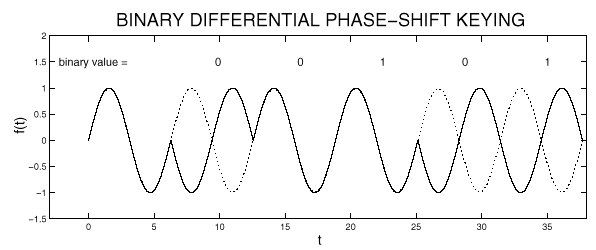
\includegraphics[width=1\textwidth]{./images/dbpsk.jpg}
\label{dbpsk}
\end{figure}
Na obrázku \ref{dbpsk} je znázorněn příklad fungování této modulace. Pokud nenastává žádná změna ve fázi signálu identifikujme 1 pokud změna nastane pak je symbol určen jako 0. V tomto příkladu každý symbol trvá jednu periodu signálu a to by při frekvenci 868 MHz kterou Sigfox v evropě používá znamenalo přenosovou rychlost 868Mb/s což nejen nedává smysl pro daný účel, ale navíc tak Sigfox ani ve skutečnosti fungovat nemůže kvůli nemožnosti dekódobat podobný signál na jakoukoliv použitelnou vzdálenost.\\
Verze DBPSK Sigofxem používaná pro každý symbol sadu period signálu a hodnotu symbolu určí podle toho zda se průběhu vysílání této sady změní fáze (0) či nikoliv (1). Demodulace tak není tolik ovlivněna lokální proměností fáze.\\
V případě evropské verze je přenosová rychlst uplinku 100 bit/s a frekvence signálu 868,1 Mhz. Z toho vyplívá že každý bit/symbol odpovídá 8 681 000 periodám. Velké množství period využívá příjimač pro statistické určení posunu fáze každého bitu. V případě 1 bude celá sada mít fázi stejnou a v případě 0 se fáze v prostřed posune. \\
\begin{figure}
\caption{Modulace amplitudy při změně fáze \ref{https://www.disk91.com/2017/technology/sigfox/the-sigfox-radio-protocol/}}
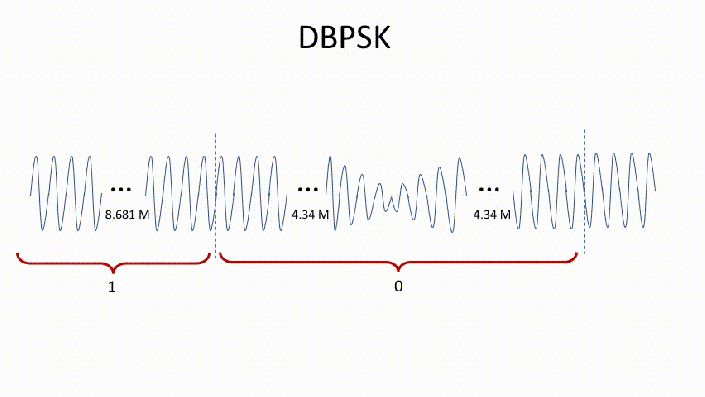
\includegraphics[width=1\textwidth]{./images/dbpsk_sigfox.jpg}
\label{dbpsk_sigfox}
\end{figure}
Pokud by se však fáze posunula při plné amplitudě znamenalo by to velký negativní dopad na spektrální efektivitu. Aby se tento efekt zmenšil je také okolo posunu fáze modulována amplituda. Grafické znázornění této modulace je na obrázku \ref{dbpsk_sigfox}.\\

\subsection{Struktura rámce uplinku}
Na fyzické vrstě Sigfox definuje rámec jako strukturu složenou z následujících polí. Pole jsou uvedena ve stejném pořadí jako v rámci. V prvním opakování není použito žádné specifické kódování a data tak jsou přímo čitelná. V druhém a třetím opakování jsou však pole F.TYPE, SEQ.ID, DEVICE.ID a PAYLOAD zakódovány.\\
Při druhém opakování hodnota každého bitu závisí na dvou předchozích, pokud jsou stejné tak je hodnota aktualního bitu prohozena. Při třetím opakování závisí hodnota aktuálních dvou bitů vždy na hodnotě dvou předchozích !!!!!!!! uplne nevim jak !!!! možná jen tak, že pokud je objeden dozadu nula tak prohazuji hodnotu.\\
Následkem použití jiného kódování pro každé opakování, není i přes identický obsah nikdy vysílán stejný rámec třikrát. Změny fáze jsou vždy na jiných místech, to může pomoci při přijmu zejména v podmínkách kdy se signál ztrácí v šumu.\\
Speciálním typem rámce uplinku je rámec OOB (Out of Band) který slouží jako potvrzení příjmu rámce downlinku. Lyší se v několika ohledech, jednak není opakován a druhak nepřenáší uživatelsky užitečná data. Místo nich v PAYLOAD poli, které je vždy dlouhé 8 bajtů, zasílá informace o napětí během nečinosti i během vysílání, teplotu, RX RSSI.

\begin{figure}
\caption{Struktura rámce Sigfox pro Uplink (nahoře) a konkrétní podoba rámce OOB (dole). Každá buňka reprezentuje půslabiku (4 bity)}
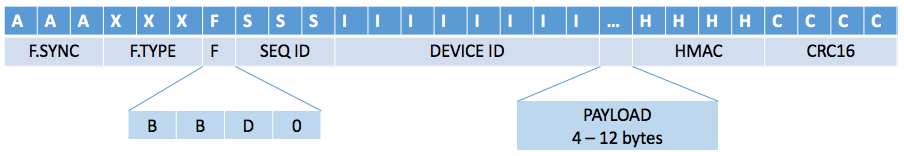
\includegraphics[width=1\textwidth]{./images/SigfoxFrameRx.png}
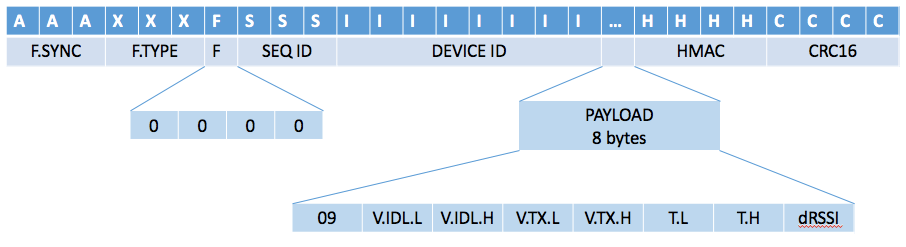
\includegraphics[width=1\textwidth]{./images/SigfoxFrameOobRx.png}
\label{sigfoxRxRamce}
\end{figure}

\begin{description}
\item[F.SYNC]
Nebo také Frame Synchronization jak již název napovídá slouží pro synchronizaci. Objevuje se na začátku každého rámce. V rámci této části se střídá 0 a 1 po dobu 3 půlslabik (12 bitů), objevuje se tedy 6 změn fáze. Tyto změny fáze využívá příjímač k synchronizaci hodin aby později korektně identifikoval začátek každého bitu.\\
Synchronizace je ukončena ve chvíli, kdy se vzor změní z 01 na 00 nebo 11 v závislosti na typu rámce. Typ rámce je určen v následujícím poli F.TYPE.

\begin{table}[]
\begin{tabular}{@{}llll@{}}
\toprule
Délka zprávy & 1. opakování & 2. opakování & 3. opakování \\ \midrule
12 bajtů     & 0x94C        & 0x971        & 0x997        \\
8 bajtů      & 0x611        & 0x6BF        & 0x72C        \\
4 bajty      & 0x35F        & 0x598        & 0x5A3        \\
1 bajt       & 0x08D        & 0x0D2        & 0x302        \\
1 bit        & 0x06B        & 0x6E0        & 0x034        \\
RX OOB       & 0xF67        & -            & -            \\ \bottomrule
\end{tabular}
\caption{Hodnoty F.TYPE v závislosti na délce zprávy a pořadí opakování}
\label{tab:ftype}
\end{table}

\item[F.TYPE]
Frame Type je část rámce, dle které lze rozeznat o kolikáté opakování (každý rámec se opakuje třikrát) vysílání se jedná a také délku užitečných dat. Přesné hodnoty nejsou nikde definovány, ale z pokusů o reverzní inženýrství \ref{https://www.disk91.com/2017/technology/sigfox/the-sigfox-radio-protocol/comment-page-1/#comment-398580} vyplývá tabulka \ref{tab:ftype}. (mohu/nemohu potvrdit) Zajímavé je, že opakování a délka dat nemají samostatné indikační bity, ale existují konstanty pro jejich kombinace.
\item[F.FLAGS]
Tato půslabika je rozdělená do tří částí. První dva bity určují počet bajtů přidaných do rámce jako výplň pro dosažení jedné z předdefinovaných délek. To znamená, že pokud by délka zprávy vyšla na 6 bajtů, tak bude odeslána v osmi bajtovém rámci a dva bajty tak budou přidány a hodnota těchto bitů bude 10 neboli 2.\\
Třetí bit značí zda je na tento rámec vyžadována odpověď ve formě downlinku. Pokud je tento bit 1 síť by měla v následujícím intervalu pro downlink odpovědět. Poslední bit je vždy 0.\\
V případě OBB rámce jsou všechny bity 0.
\item[SEQ.ID]
Sequence ID je 12 bitové pole, které se inkrementuje s každým odeslaným rámcem. Slouží jako určitá ochrana proti znovuodeslání zachycených zpráv. Limitem této ochrany je, že se SEQ.ID každých 2048 zpráv opakuje a tak v určitých situacích nemusí backend znovuodeslanou zprávu zachytit. Bity jsou seřazeny od nejvýznamějšího po nejméně významný.
\item[DEVICE.ID]
Toto pole je dlouhé 32 bitů a představuje unikátní ID Sigfox zařízení. Bajty jsou řazeny od nejméně významného, ale bity každého z nich jsou řazeny od nejvýznamějšího bitu.
\item[PAYLOAD]
Toto pole obsahuje přenášená data a může být dlouhé 12, 8 nebo 4 bajty.
\item[HMAC]
HMAC (hash-based message authentication code) je druh MAC projejíž výpočet je použitá kryptografická hešovací funkce a tajný klíč. Slouží jak ke kontrole integrity dat, tak k autentifikaci. Každé Sigfox zařízení má svůj tajný privátní klíč vypálený přímo na čipu. Délka pole je 2 bajty.
\item[CRC]
Poslední pole je CRC s délkou 16 bitů.
\end{description}

\subsection{Downlink}
Pro komunikaci směrem ze sítě do zařízení Sigfox používá modulační schéma GFSK, vyšší výkon, širší pásmo a navíc má i větší poměr vysílacího času, viz \ref{tab:upAndDown}. Mohlo by se zdát, že jsou Uplink a Downlink kanály nevyvážené ve prospěch Downlinku, ale opak je pravdou jelikož Downlink je vysílán pro všechna zařízení v dosahu a Uplink se počítá pro každé zařízení zvlášť. V Evropě po započtení všech omezení vychází pro každé zařízení 140 Uplink zpráv denně a jen 4 Downlink zprávy.\\
Přesný obsah rámce ani další detaily momentálně neznám. Pouze lze něco málo vyčíst z tabulky \ref{tab:downlinkFrame}.
\begin{table}[]
\begin{tabular}{@{}|l|l|l|l|l|l|@{}}
\toprule
Preamble (91) & Frame Sync (13) & ECC (32) & Payload (0 - 64) & MAC (16) & FCS (8) \\ \bottomrule
\end{tabular}
\caption{Pole rámce Downlinku (délka pole v bitech)}
\label{tab:downlinkFrame}
\end{table}

\chapter{Závěr}

Lorep ipsum \cite{doe}

\begin{thebibliography}{1}

\bibitem{doe} J. Doe. \emph{Book on foobar.} Publisher X,
 2300.

\end{thebibliography}

\end{document}
